\chapter{الانتقاء والانسياق والانتواع}\label{ch:g12:selection-drift-speciation}

في سنة 1848 اصطيدت صورة سوداء من عثة الفلفل قرب مدينة صناعية كان كل
جذع شجرة فيها مطليًا بالسخام؛ وبحلول سنة 1895 صارت كل عثة في المنطقة
تقريبًا سوداء. وبعد قرن، وقد زال السخام وعادت الجذوع فاتحة، كادت الصورة
السوداء تختفي. ولم يرب أحد تلك العث؛ بل قامت بالفرز الطيور التي تأكلها.
وقد وصف الفصلان الماضيان كيف ينشأ التنوع؛ وهذا الفصل في ما يحل به داخل
\omterm{def:g12:selection-drift-speciation:population}{جمهرة} --- كيف تشيع بعض \omterm{def:g10:universal-dna:gene}{الأليلات} وتندر أخرى، بالانتقاء وبالمصادفة ---
وكيف تصير \omterm{def:g12:selection-drift-speciation:population}{جمهرة} واحدة، في النهاية، نوعين.

\section{الجمهرات وأليلاتها}

\begin{definition}[الجمهرة وتواتر الأليل]\label{def:g12:selection-drift-speciation:population}
\emph{الجمهرة}\index{جمهرة} طقم أفراد \omterm{def:g10:biodiversity-scales:species}{النوع} الواحد الذين يعيشون في
المكان نفسه ويتناسلون فيما بينهم. ويوصف تركيبها الوراثي بذكر
\emph{تواترات}\index{تواتر أليلي} \omterm{def:g10:universal-dna:gene}{أليلات} كل \omterm{def:g10:universal-dna:gene}{مورّثة}: فلمورّثة لها
أليلان $A$ و$a$، الكسر $p$ من النسخ كلها هو ما كان $A$، والكسر
$q = 1 - p$ هو ما كان $a$. والتطور، على هذا المقياس، تغير في تواترات
\omterm{def:g10:universal-dna:gene}{الأليلات} من جيل إلى جيل.
\end{definition}

\begin{proposition}[التواترات بلا أي قوة]\label{prop:g12:selection-drift-speciation:hw}
في \omterm{def:g12:selection-drift-speciation:population}{جمهرة} كبيرة يقع فيها التزاوج عشوائيًا، ولا يعطي فيها أي \omterm{def:g10:universal-dna:gene}{أليل} ميزة،
ولا تقع فيها \omterm{def:g11:mutations:mutation}{طفرة} ولا هجرة، تبقى \omterm{def:g12:selection-drift-speciation:population}{تواترات} \omterm{def:g10:universal-dna:gene}{الأليلات} على حالها من جيل إلى
جيل، وتظهر الأنماط الوراثية بالنسب
\[
AA : Aa : aa = p^2 : 2pq : q^2 .
\]
وهذه هي الحالة المرجعية: فأي خروج عنها، يلاحظ عبر الأجيال، دليل على أن
أحد الشروط قد سقط --- أي أن الانتقاء أو المصادفة أو الهجرة أو \omterm{def:g11:mutations:mutation}{الطفرة}
يعمل.
\end{proposition}
\begin{proof}
كل مشيج يحمل $A$ باحتمال $p$ ويحمل $a$ باحتمال $q$؛ ومشيجان يسحبان
عشوائيًا يعطيان $AA$ باحتمال $p^2$، و$aa$ باحتمال $q^2$، و$Aa$ باحتمال
$pq + qp = 2pq$. وبإحصاء \omterm{def:g10:universal-dna:gene}{أليلات} الجيل الجديد: تؤلف نسخ $A$ مقدار
$p^2 + \tfrac12 (2pq) =
p(p + q) = p$ من المجموع. فالتواتر لم يتغير.
\end{proof}

\begin{omfigure}
\begin{tikzpicture}[font=\small]
  \draw[thick] (0,0) rectangle (5,5);
  \fill[omDef!25] (0,1.5) rectangle (3.5,5);
  \fill[omProp!25] (3.5,1.5) rectangle (5,5);
  \fill[omProp!25] (0,0) rectangle (3.5,1.5);
  \fill[omThm!30] (3.5,0) rectangle (5,1.5);
  \draw (3.5,0) -- (3.5,5); \draw (0,1.5) -- (5,1.5);
  \node at (1.75,3.25) {$AA$: $p^2$}; \node at (4.25,3.25) {$Aa$: $pq$};
  \node at (1.75,0.75) {$Aa$: $pq$}; \node at (4.25,0.75) {$aa$: $q^2$};
  \node[anchor=south] at (1.75,5.1) {$A$، بتواتر $p$}; \node[anchor=south] at (4.25,5.1) {$a$، $q$};
  \node[anchor=east] at (-0.1,3.25) {$A$, $p$}; \node[anchor=east] at (-0.1,0.75) {$a$, $q$};
  \node[anchor=south, font=\small\itshape] at (2.5,5.6) {مشيج الأب};
  \node[font=\small\itshape, rotate=90, anchor=south] at (-1.1,2.5) {مشيج الأم};
  \node[anchor=west, align=left, text width=6cm] at (6,2.5) {مع $p = 0.7$ و$q = 0.3$: $AA$ 49\%، و$Aa$ 42\%، و$aa$ 9\%. فصفة متنحية تبديها 9\% من جمهرة تحملها، في صمت، 42\% أخرى.};
\end{tikzpicture}

{\small نسب الأنماط الوراثية في التزاوج العشوائي، ممثلة مساحات. فضلعا
المربع تواترا المشيجين؛ والمستطيلات الأربعة الأنماط الوراثية. ومتغايرو
\omterm{def:g10:universal-dna:gene}{الأليلين} يحوزون معظم نسخ \omterm{def:g10:universal-dna:gene}{الأليل} النادر.}
\end{omfigure}

\begin{example}[إحصاء الأليلات]\label{ex:g12:selection-drift-speciation:count}
بين 1000 شخص، 490 منهم $AA$، و420 $Aa$، و90 $aa$. فنسخ $a$:
$420 + 2 \times 90 = 600$ من 2000، ومن ثم $q = 0.3$ و$p = 0.7$ ---
وأعداد الأنماط الوراثية هي بالضبط $p^2$ و$2pq$ و$q^2$ من 1000:
\omterm{def:g12:selection-drift-speciation:population}{فالجمهرة} في الحالة المرجعية عند هذه \omterm{def:g10:universal-dna:gene}{المورّثة}. ومرض \omterm{def:g11:genes-and-disease:genetic}{متنح} يصيب مولودًا
واحدًا من كل 2500 ($q^2 = 1/2500$) يستلزم $q = 1/50$ وحاملين
$2pq \approx 1/25$: وهي أرقام \cref{ch:g11:genes-and-disease}، مستنتجة.
\end{example}

\section{الانتقاء}

\begin{definition}[الانتقاء الطبيعي]\label{def:g12:selection-drift-speciation:selection}
\emph{الانتقاء الطبيعي}\index{انتقاء طبيعي} هو الفرق في التناسل بين
الأفراد الحاملين \omterm{def:g10:universal-dna:gene}{أليلات} مختلفة، في بيئة بعينها: فحملة \omterm{def:g10:universal-dna:gene}{أليل} يخلّفون،
وسطيًا، نسلًا أكثر من حملة \omterm{def:g10:universal-dna:gene}{أليل} آخر، فيرتفع تواتر \omterm{def:g10:universal-dna:gene}{الأليل} من جيل إلى
جيل. والمنتقى هو الفرد كله --- بقاؤه، وتزاوجه، وخصوبته --- \omterm{def:g10:universal-dna:gene}{والأليلات}
تركب معه.
\end{definition}

\begin{proposition}[الانتقاء يغير التواترات في اتجاه]\label{prop:g12:selection-drift-speciation:direction}
\omterm{def:g10:universal-dna:gene}{الأليل} الذي يحظى حملته بنجاح تناسلي أعلى ولو قليلًا ينتشر؛ والذي يحظى
حملته بأقل يندر. والاتجاه تحدده البيئة، وينعكس إن انعكست؛ والسرعة تتوقف
على حجم الميزة وعلى هل يعبَّر عن \omterm{def:g10:universal-dna:gene}{الأليل} في نسخة واحدة (\omterm{def:g11:genes-and-disease:genetic}{سائد}، فسريع) أم
في نسختين لا غير (\omterm{def:g11:genes-and-disease:genetic}{متنح}، فبطيء في البدء، ولا يزال أبدًا زوالًا تامًا، إذ
تختبئ نسخه النادرة في متغايري \omterm{def:g10:universal-dna:gene}{الأليلين}).
\end{proposition}
\begin{proof}[شواهد]
عثة الفلفل: تأخذ الطيور ما تراه من العث؛ فعلى الجذوع المسخمة ترى
الصورة الفاتحة، وعلى النظيفة ترى الصورة الداكنة؛ وقد ارتفع تواتر
\omterm{def:g10:universal-dna:gene}{الأليل} الداكن من قرب الصفر إلى 98\% في خمسين سنة من التلوث، ثم عاد
فهبط دون 10\% في أربعين سنة من الهواء النقي، متتبعًا الجذوع. \omterm{prop:g11:antibiotic-resistance:mechanisms}{ومقاومة
المضادات الحيوية} (\cref{ch:g11:antibiotic-resistance}): فحملة \omterm{def:g10:universal-dna:gene}{الأليل}
المقاوم وحدهم يتناسلون بحضور الدواء. ودوام اللاكتاز
(\cref{ch:g11:enzymes-and-phenotype}): \omterm{def:g10:universal-dna:gene}{فالأليل} شائع بالضبط حيث كان
الحليب غذاء للبالغين آلاف السنين. وفي كل حالة يتبع حظ \omterm{def:g10:universal-dna:gene}{الأليل} البيئة.
\end{proof}

\begin{omfigure}
\begin{tikzpicture}
\begin{axis}[
  width=0.88\linewidth, height=5.6cm,
  axis x line=bottom, axis y line=left,
  xmin=1840, xmax=2000, ymin=0, ymax=110,
  xlabel={السنة}, ylabel={العث الداكن (\% من المصائد)},
  xlabel style={font=\small, at={(axis description cs:0.5,-0.12)}, anchor=north},
  ylabel style={font=\small},
  tick label style={font=\small}, xtick={1850,1875,1900,1925,1950,1975,2000}, ytick={0,25,50,75,100},
  clip=false,
]
\addplot[thick, omThm, mark=*, mark size=1.3pt] coordinates
  {(1848,1) (1860,10) (1870,40) (1880,75) (1895,98) (1920,97) (1950,95) (1960,90) (1970,60) (1980,30) (1990,10) (1998,4)};
\draw[dashed, gray] (axis cs:1956,0) -- (axis cs:1956,105);
\node[font=\scriptsize, anchor=south] at (axis cs:1956,105) {قوانين نقاء الهواء};
\end{axis}
\end{tikzpicture}

{\small تواتر الصورة الداكنة من عثة الفلفل قرب مدينة صناعية (مدوَّرًا
من مجموعات المتاحف والمصائد). فالارتفاع يتتبع اسوداد الجذوع، والهبوط
يتتبع تنظيفها. وقد انعكس الانتقاء حين انعكست البيئة.}
\end{omfigure}

\begin{omfigure}
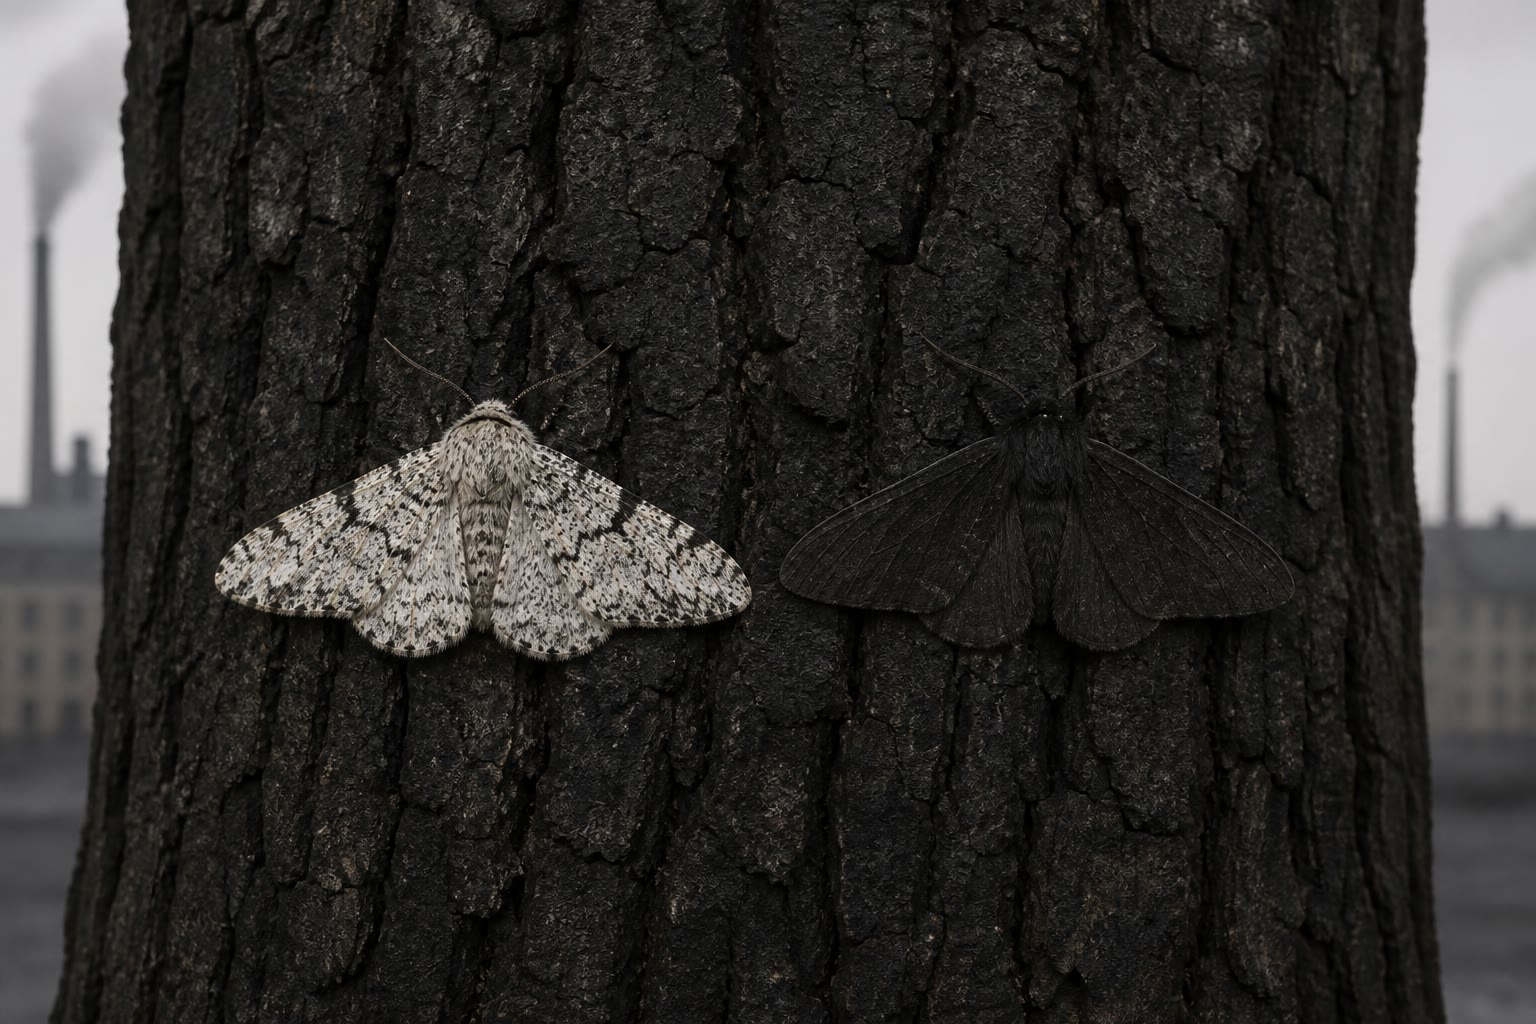
\includegraphics[width=0.6\linewidth]{images/book2/ai/g12-selection-peppered-moths.jpg}

{\small صورتا عثة الفلفل على جذع أسودّ بالسخام. والطيور تصطاد بالبصر:
فعلى هذا اللحاء تؤخذ الصورة الفاتحة وتنجو الداكنة؛ وعلى جذع نظيف مكسو
بالأشنات يكون العكس.}
\end{omfigure}

\begin{example}[انتقاء الجنس الآخر]\label{ex:g12:selection-drift-speciation:sexual}
ذيل الطاووس يجعله أبطأ وأظهر للمفترسات، ومع ذلك يبقى لأن الإناث تختار
الذكور ذوي الذيول الأكبر والأنظم: \omterm{def:g10:universal-dna:gene}{فالأليل} الذي يحسّن الذيل ينقل أكثر،
مهما كلّف من بقاء. و\emph{الانتقاء الجنسي} --- أي اختيار القرناء ---
ينتج زينة الحيوان وأغانيه ومنازلاته، ويستطيع أن يدفع صفة في اتجاه ما
كان البقاء وحده ليحبذه أبدًا.
\end{example}

\section{المصادفة: الانسياق الوراثي}

\begin{proposition}[الانسياق الوراثي]\label{prop:g12:selection-drift-speciation:drift}
في أي \omterm{def:g12:selection-drift-speciation:population}{جمهرة} منتهية الحجم، تكون \omterm{def:g10:universal-dna:gene}{أليلات} جيل عينة عشوائية من \omterm{def:g10:universal-dna:gene}{أليلات} الجيل
السابق: فأي الأفراد يتصادف أن يتناسل، وأي \omterm{def:g10:universal-dna:gene}{الأليلات} يتصادف أن تحملها
أمشاجه، أمران يتذبذبان بالمصادفة. ومن ثم تهيم \omterm{def:g12:selection-drift-speciation:population}{تواترات} \omterm{def:g10:universal-dna:gene}{الأليلات} من جيل
إلى جيل من غير أن تدخل أي ميزة --- وهو \emph{الانسياق
الوراثي}\index{انسياق وراثي}. وكلما صغرت \omterm{def:g12:selection-drift-speciation:population}{الجمهرة} كبر الهيام؛ ففي \omterm{def:g12:selection-drift-speciation:population}{جمهرة}
صغيرة يستطيع \omterm{def:g10:universal-dna:gene}{أليل} أن يضيع، أو أن يبلغ 100\%، بالمصادفة وحدها في غضون
أجيال قليلة، أيًا كانت قيمته.
\end{proposition}
\begin{proof}[شواهد]
\omterm{def:g12:selection-drift-speciation:population}{الجمهرات} التي يؤسسها أفراد قلائل --- كجزيرة استعمرتها حفنة من الطيور،
أو جماعة بشرية منحدرة من بضع عشرات من المستوطنين --- تحمل عينة مشوَّهة
من \omterm{def:g10:universal-dna:gene}{أليلات} \omterm{def:g12:selection-drift-speciation:population}{الجمهرة} الأصل: فقد يشيع فيها \omterm{def:g10:universal-dna:gene}{أليل} مرض نادر، ويغيب كثير من
تنوع الأصل. \omterm{def:g10:biodiversity-scales:species}{والأنواع} التي مرت
\emph{بعنق زجاجة} من ناجين قلائل جدًا (كالفهد في
\cref{ch:g10:biodiversity-scales}، وفيل البحر الشمالي الذي انحدر
إلى عشرين حيوانًا سنة 1890) لا تكاد تبدي اليوم تنوعًا وراثيًا،
حتى بعد أن تعافت إلى الألوف. وفي المختبر، تتبعثر \omterm{def:g12:selection-drift-speciation:population}{جمهرات} صغيرة كثيرة
متماثلة بدئت عند التواتر نفسه في كل اتجاه في غضون أجيال قليلة، بينما
تثبت الكبيرة مكانها.
\end{proof}

\begin{omfigure}
\begin{tikzpicture}
\begin{axis}[
  width=0.88\linewidth, height=5.8cm,
  axis x line=bottom, axis y line=left,
  xmin=0, xmax=20, ymin=0, ymax=1.05,
  xlabel={الجيل}, ylabel={تواتر الأليل $A$},
  xlabel style={font=\small, at={(axis description cs:0.5,-0.12)}, anchor=north},
  ylabel style={font=\small},
  tick label style={font=\small}, xtick={0,5,10,15,20}, ytick={0,0.25,0.5,0.75,1},
  legend style={at={(0.5,-0.3)}, anchor=north, legend columns=2, font=\small, draw=none},
]
\addplot[thick, omThm] coordinates {(0,0.5) (1,0.55) (2,0.6) (3,0.5) (4,0.65) (5,0.7) (6,0.6) (7,0.75) (8,0.85) (9,0.8) (10,0.9) (11,0.95) (12,1) (13,1) (14,1) (15,1) (16,1) (17,1) (18,1) (19,1) (20,1)};
\addplot[thick, omThm!60] coordinates {(0,0.5) (1,0.4) (2,0.45) (3,0.3) (4,0.35) (5,0.25) (6,0.3) (7,0.2) (8,0.1) (9,0.15) (10,0.05) (11,0.1) (12,0) (13,0) (14,0) (15,0) (16,0) (17,0) (18,0) (19,0) (20,0)};
\addplot[thick, omThm!35] coordinates {(0,0.5) (1,0.45) (2,0.55) (3,0.6) (4,0.5) (5,0.4) (6,0.45) (7,0.55) (8,0.6) (9,0.7) (10,0.65) (11,0.55) (12,0.5) (13,0.6) (14,0.65) (15,0.75) (16,0.7) (17,0.8) (18,0.75) (19,0.85) (20,0.8)};
\addplot[thick, omDef] coordinates {(0,0.5) (1,0.51) (2,0.49) (3,0.5) (4,0.52) (5,0.51) (6,0.5) (7,0.49) (8,0.48) (9,0.49) (10,0.5) (11,0.51) (12,0.52) (13,0.51) (14,0.5) (15,0.5) (16,0.49) (17,0.5) (18,0.51) (19,0.5) (20,0.5)};
\legend{{ثلاث جمهرات من 20}, {جمهرة من 5000}}
\end{axis}
\end{tikzpicture}

{\small انسياق محاكى \omterm{def:g10:universal-dna:gene}{لأليل} حيادي يبدأ عند 50\%. ففي \omterm{def:g12:selection-drift-speciation:population}{جمهرات} من 20 فردًا
يثبَّت أو يضيع في غضون اثني عشر جيلًا، في اتجاه مختلف في كل مرة؛ وفي
\omterm{def:g12:selection-drift-speciation:population}{جمهرة} من 5000 لا يكاد يتحرك.}
\end{omfigure}

\begin{example}[أثر المؤسس]\label{ex:g12:selection-drift-speciation:founder}
جماعة في جزيرة أسسها بضع عشرات من المستوطنين، أحدهم يحمل \omterm{def:g10:universal-dna:gene}{أليل} اضطراب
نادر في العين. وبعد عشرة أجيال صار تواتر \omterm{def:g10:universal-dna:gene}{الأليل} في الجماعة واحدًا من
كل عشرة --- أي مئة ضعف قيمته في البر --- لأن حاملًا واحدًا بين ثلاثين
مؤسسًا هو أصلًا 1.7\% من النسخ، ولأن الانسياق في \omterm{def:g12:selection-drift-speciation:population}{جمهرة} صغيرة معزولة
دفعه أبعد. \omterm{def:g10:universal-dna:gene}{والأليل} لا يمنح أي ميزة؛ ووفرته حادثة عارضة تخص من ركب
المركب.
\end{example}

\begin{method}[انتقاء أم انسياق؟]\label{met:g12:selection-drift-speciation:which}
إذا واجهت تغيرًا في تواتر \omterm{def:g10:universal-dna:gene}{أليل}:
\begin{enumerate}
  \item قدّر حجم \omterm{def:g12:selection-drift-speciation:population}{الجمهرة}: فالانسياق قوي دون بضع مئات، ومهمل في
        الملايين.
  \item ابحث عن اتجاه يتتبع البيئة (انتقاء)، أو عن مشية عشوائية
        (انسياق). \omterm{def:g12:selection-drift-speciation:population}{فالجمهرات} المتماثلة إن تحركت في الاتجاه نفسه دلت على
        انتقاء؛ وإن تحركت في اتجاهات مختلفة دلت على انسياق.
  \item ابحث عن آلية تربط \omterm{def:g10:universal-dna:gene}{الأليل} بالبقاء أو بالتناسل؛ فإن لم تجد
        فاشتبه بالانسياق.
  \item وتذكر أنهما يعملان معًا: فالانتقاء يرسم ميلًا، والانسياق يضيف
        ضجيجًا، وفي \omterm{def:g12:selection-drift-speciation:population}{الجمهرات} الصغيرة قد يغرق الضجيج الميل.
\end{enumerate}
\end{method}

\section{من الجمهرة إلى النوع}

\begin{proposition}[الانتواع]\label{prop:g12:selection-drift-speciation:speciation}
جمهرتان من \omterm{def:g10:biodiversity-scales:species}{نوع} واحد تكفان عن تبادل \omterm{def:g10:universal-dna:gene}{المورّثات} --- يفصلهما حاجز من
جغرافيا أو سلوك أو توقيت --- تتطوران متباعدتين: فتراكم كل منهما
طفراتها، وتنتقيها بيئتها، وتنساق سبيلها. فإذا بلغ التباعد مبلغًا لم
يعد معه أفراد الجمهرتين يتناسلون، أو صاروا يعطون نسلًا عقيمًا، ولو
التقوا ثانية، وجد نوعان حيث كان \omterm{def:g10:biodiversity-scales:species}{نوع} واحد. و\emph{الانتواع}\index{انتواع}
هو هذا المسار؛ وهو يأخذ عادة من آلاف الأجيال إلى ملايينها، وإن كان
\omterm{prop:g12:diversification-of-life:polyploidy}{تعدد الصيغ الصبغية} (\cref{ch:g12:diversification-of-life}) يبلغه في
جيل واحد.
\end{proposition}
\begin{proof}[شواهد]
جزر غالاباغوس: كل جزيرة منها تحمل عصافيرها، منحدرة من \omterm{def:g10:biodiversity-scales:species}{نوع} بري
وأقرب ما تكون إلى عصافير الجزيرة المجاورة. والبحيرات: سمكة بلطية سلفية
واحدة أعطت مئات \omterm{def:g10:biodiversity-scales:species}{الأنواع} في بحيرة أفريقية واحدة في غضون بضع مئات من
الألوف من السنين، يفصلها الموئل واختيار الإناث للون الذكر. \omterm{def:g10:biodiversity-scales:species}{والأنواع}
الحلقية: \omterm{def:g12:selection-drift-speciation:population}{جمهرات} نورس انتشرت حول القطب الشمالي، يتناسل بعضها مع جيرانه
على طول الطريق حتى يلتقي الطرفان في أوروبا صورتين لا تتناسلان --- أي
حد نوعي أمسك به وهو يتكون. \omterm{def:g10:biodiversity-scales:species}{والأنواع} التي انفصلت حديثًا، كالدب القطبي
والدب البني، ما زالت تنتج هجنًا خصيبة أحيانًا: فالحد مسألة درجة.
\end{proof}

\begin{omfigure}
\begin{tikzpicture}[font=\small, >=Stealth]
  % one population
  \draw[thick, fill=omDef!12] (0,0) ellipse (1.4 and 0.8);
  \node at (0,0) {جمهرة واحدة};
  \draw[->, thick] (1.6,0) -- (2.6,0) node[midway, above, font=\scriptsize, align=center] {يظهر\\ حاجز};
  % two separated
  \draw[thick, fill=omDef!12] (4.0,0.9) ellipse (1.2 and 0.6); \node at (4.0,0.9) {جمهرة 1};
  \draw[thick, fill=omDef!12] (4.0,-0.9) ellipse (1.2 and 0.6); \node at (4.0,-0.9) {جمهرة 2};
  \draw[very thick, gray] (2.7,0) -- (5.3,0);
  \draw[->, thick] (5.5,0) -- (6.5,0) node[midway, above, font=\scriptsize, align=center] {تطور\\ منفصل};
  % diverged
  \draw[thick, fill=omMeth!15] (7.9,0.9) ellipse (1.2 and 0.6); \node at (7.9,0.9) {طفرات 1};
  \draw[thick, fill=omThm!15] (7.9,-0.9) ellipse (1.2 and 0.6); \node at (7.9,-0.9) {طفرات 2};
  \node[font=\scriptsize, align=center] at (7.9,0.0) {انتقاء خاص،\\ وانسياق خاص};
  \draw[->, thick] (9.3,0) -- (10.3,0) node[midway, above, font=\scriptsize, align=center] {يزول\\ الحاجز};
  % two species
  \draw[thick, fill=omMeth!15] (11.6,0.7) ellipse (1.1 and 0.55); \node at (11.6,0.7) {نوع 1};
  \draw[thick, fill=omThm!15] (11.6,-0.7) ellipse (1.1 and 0.55); \node at (11.6,-0.7) {نوع 2};
  \node[font=\scriptsize, align=center] at (11.6,0.0) {لا تناسل بينهما};
\end{tikzpicture}

{\small \omterm{prop:g12:selection-drift-speciation:speciation}{الانتواع} بالفصل. حاجز يشق \omterm{def:g12:selection-drift-speciation:population}{جمهرة}؛ فيتطور كل نصف على حدة؛ فإذا
التقيا ثانية لم يتناسلا. وقد يكون الحاجز مضيقًا أو جبلًا أو تغير موئل
أو تفضيلًا في التزاوج.}
\end{omfigure}

\begin{proposition}[النوع، معادًا فيه النظر]\label{prop:g12:selection-drift-speciation:concept}
\omterm{def:g10:biodiversity-scales:species}{النوع} \omterm{def:g12:selection-drift-speciation:population}{جمهرة}، أو طقم \omterm{def:g12:selection-drift-speciation:population}{جمهرات}، يتناسل أفرادها فيما بينهم ويعزلون وراثيًا
عن سائر تلك الأطقم --- وهو تعريف ينفع في معظم الحيوان والنبات في لحظة
بعينها، لكن له حوافّ: \omterm{def:g12:selection-drift-speciation:population}{كالجمهرات} وهي في طريق الانفصال، \omterm{def:g10:biodiversity-scales:species}{والأنواع} التي ما
زالت تتهاجن، والكائنات التي تتكاثر بلا جنس. \omterm{def:g10:biodiversity-scales:species}{والنوع} ليس نمطًا ثابتًا بل
سلالة في الزمن: يبدأ حين تعزل \omterm{def:g12:selection-drift-speciation:population}{جمهرة}، ويوجد ما دام أفراده يتناسلون،
وينتهي بالانقراض أو بالانشقاق إلى \omterm{def:g10:biodiversity-scales:species}{أنواع} جديدة. \omterm{def:g10:biodiversity-scales:species}{والأنواع} الحية اليوم
أطراف شجرة أفرعها موضوع \cref{ch:g12:phylogenetic-trees}.
\end{proposition}
\admitted

\begin{remark}[التطور، مجموعًا]\label{rem:g12:selection-drift-speciation:assembled}
\omterm{def:g11:mutations:mutation}{الطفرة} والخلط يمدان بالتنوع؛ والتضاعف والنقل \omterm{prop:g12:diversification-of-life:polyploidy}{وتعدد الصيغ الصبغية}
والتنظيم \omterm{def:g12:diversification-of-life:symbiosis}{والتعايش} تمد بمزيد؛ والانتقاء يفرزه بالبيئة، والانسياق
بالمصادفة؛ والعزل يدع \omterm{def:g12:selection-drift-speciation:population}{الجمهرات} تتباعد حتى تصير أنواعًا؛ والانقراض
يزيلها. وليس لأي من هذه الخطوات غاية، ولا واحدة منها تنظر إلى الأمام؛
لكنها معًا، على مدى أربعة مليارات من السنين من السجل الأحفوري، أنتجت
تنوّع \cref{ch:g10:biodiversity-scales}. والنظرية التي تسمي هذه
الخطوات وتفاعلها هي نظرية التطور، وكل فصل من فصول هذه السنة كان قطعة
من شواهدها.
\end{remark}

\section{تمارين}

\begin{exercise}[$\star$]\label{exo:g12:selection-drift-speciation:1}
عرّف تواتر \omterm{def:g10:universal-dna:gene}{الأليل}، وأعط نسب الأنماط الوراثية في \omterm{def:g12:selection-drift-speciation:population}{جمهرة} في الحالة
المرجعية عند $p = 0.8$.
\end{exercise}

\begin{exercise}[$\star$]\label{exo:g12:selection-drift-speciation:2}
عرّف \omterm{def:g12:selection-drift-speciation:selection}{الانتقاء الطبيعي} \omterm{prop:g12:selection-drift-speciation:drift}{والانسياق الوراثي}، واذكر الفرق الجوهري بينهما.
\end{exercise}

\begin{exercise}[$\star$]\label{exo:g12:selection-drift-speciation:3}
من شكل العث، اقرأ تواتر الصورة الداكنة سنة 1880 وسنة 1980، وسمّ التغير
البيئي وراء كل منهما.
\end{exercise}

\begin{exercise}[$\star$]\label{exo:g12:selection-drift-speciation:4}
لماذا كان الانسياق أهم في \omterm{def:g12:selection-drift-speciation:population}{جمهرة} صغيرة؟
\end{exercise}

\begin{exercise}[$\star$]\label{exo:g12:selection-drift-speciation:5}
ما اللازم لتصير \omterm{def:g12:selection-drift-speciation:population}{جمهرة} واحدة نوعين؟
\end{exercise}

\begin{exercise}[$\star\star$]\label{exo:g12:selection-drift-speciation:6}
في \omterm{def:g12:selection-drift-speciation:population}{جمهرة} من 500، منهم 320 $AA$ و160 $Aa$ و20 $aa$. احسب $p$ و$q$، ثم
أعداد الأنماط الوراثية المنتظرة في الحالة المرجعية، وقارن.
\end{exercise}

\begin{exercise}[$\star\star$]\label{exo:g12:selection-drift-speciation:7}
\omterm{def:g10:universal-dna:gene}{أليل} \omterm{def:g11:genes-and-disease:genetic}{متنح} تواتره 0.01. ما كسر \omterm{def:g12:selection-drift-speciation:population}{الجمهرة} الذي يبدي الصفة المتنحية، وما
الكسر الذي يحمل \omterm{def:g10:universal-dna:gene}{الأليل} من غير أن يظهر؟ ولماذا كان \omterm{def:g10:universal-dna:gene}{الأليل} عسير الإزالة
بالانتقاء ضد الصفة؟
\end{exercise}

\begin{exercise}[$\star\star$]\label{exo:g12:selection-drift-speciation:8}
من شكل الانسياق، في كم جيلًا ثبّت \omterm{def:g10:universal-dna:gene}{الأليل} أو ضاع في الجمهرتين الصغيرتين
اللتين بلغتا الطرفين؟ ولماذا لم تفعل الثالثة؟
\end{exercise}

\begin{exercise}[$\star\star$]\label{exo:g12:selection-drift-speciation:9}
فسّر لماذا لم يبلغ \omterm{def:g10:universal-dna:gene}{الأليل} الداكن عند عثة الفلفل 100\% في عقود السخام،
مستعينًا بالعث الذي يعيش ويتناسل في الريف.
\end{exercise}

\begin{exercise}[$\star\star$]\label{exo:g12:selection-drift-speciation:10}
نجا عشرون فيلًا بحريًا من عنق زجاجة؛ وعدد \omterm{def:g10:biodiversity-scales:species}{النوع} اليوم 100\,000 ومع
ذلك لا يكاد يبدي تنوعًا وراثيًا. فسّر بالانسياق.
\end{exercise}

\begin{exercise}[$\star\star$]\label{exo:g12:selection-drift-speciation:11}
طبّق \cref{met:g12:selection-drift-speciation:which} على حالتين: \omterm{def:g10:universal-dna:gene}{أليل}
يرتفع في عشر \omterm{def:g12:selection-drift-speciation:population}{جمهرات} بحيرية منفصلة دفعة واحدة بعد وصول مفترس جديد؛
\omterm{def:g10:universal-dna:gene}{وأليل} يبلغ 80\% في \omterm{def:g12:selection-drift-speciation:population}{جمهرة} جزيرة من ثلاثين طائرًا.
\end{exercise}

\begin{exercise}[$\star\star\star$]\label{exo:g12:selection-drift-speciation:12}
في منطقة فيها ملاريا، تواتر \omterm{def:g10:universal-dna:gene}{أليل} المنجلية 0.15 مع أن أطفال $aa$ قلما
ينجون. مستعينًا بنسب الأنماط الوراثية، احسب كسور المواليد $AA$ و$Aa$
و$aa$، وفسّر كيف تبقي ميزة $Aa$ في وجه الملاريا \omterm{def:g10:universal-dna:gene}{الأليل} شائعًا رغم فقد
أفراد $aa$.
\end{exercise}

\begin{exercise}[$\star\star\star$]\label{exo:g12:selection-drift-speciation:13}
نوعان من الأسماك البلطية في بحيرة واحدة يختلفان أساسًا في لون الذكور،
وإناث كل منهما تختار لونها. وفي الماء العكر، حيث لا ترى الألوان،
يتهاجن النوعان بحرية. فما الذي يعزل النوعين، وماذا تقول حالة العكارة
عن مدى حداثة الانفصال؟
\end{exercise}

\begin{exercise}[$\star\star\star$]\label{exo:g12:selection-drift-speciation:14}
فسّر لماذا كان نورس \omterm{def:g10:biodiversity-scales:species}{الأنواع} الحلقية حجة على أن \omterm{prop:g12:selection-drift-speciation:speciation}{الانتواع} تدريجي، ولماذا
سمي الطرفان الملتقيان في أوروبا مع ذلك نوعين.
\end{exercise}

\begin{exercise}[$\star\star\star$]\label{exo:g12:selection-drift-speciation:15}
"الانتقاء يجعل الكائنات أفضل." ناقش في فقرة: أفضل في ماذا، وأين،
وقياسًا بمن؛ وماذا يضيف الانسياق والانعكاسات والانتقاء الجنسي.
\end{exercise}

\section{مسألة: فئران الجزيرة}

\begin{problem}[{مسألة نهاية الأسبوع --- جمهرة فئران في جزيرة: تحسب
تواترات أليلاتها، ويتابع انتقاء مفترس جديد، ويحاكى انسياق مستعمرة
ضئيلة، ويستشرف مولد نوع}]
\label{pb:g12:selection-drift-speciation:1}
في جزيرة صخرية، تحمل الفئران \omterm{def:g10:universal-dna:gene}{مورّثة} لون الفراء ولها أليلان: $D$
(داكن، \omterm{def:g11:genes-and-disease:genetic}{سائد}) و$d$ (فاتح). وإحصاء لألفي فأر يجد 720 فأرًا داكنًا نمطها
الوراثي $DD$، و960 داكنًا $Dd$، و320 فاتحًا $dd$.

\medskip
\noindent\textbf{القسم الأول --- \omterm{def:g12:selection-drift-speciation:population}{الجمهرة} الآن.}
\begin{enumerate}
  \item احسب تواتر $p$ \omterm{def:g10:universal-dna:gene}{للأليل} $D$ وتواتر $q$ \omterm{def:g10:universal-dna:gene}{للأليل} $d$ بإحصاء النسخ.
  \item احسب أعداد الأنماط الوراثية المنتظرة في الحالة المرجعية وقارنها
        بالإحصاء. أفي الحالة المرجعية هذه \omterm{def:g12:selection-drift-speciation:population}{الجمهرة}؟
  \item أي كسر من الفئران الداكنة حامل \omterm{def:g10:universal-dna:gene}{للأليل} $d$؟
  \item فسّر، من الجواب السابق، لماذا كان نزع كل الفئران الفاتحة من
        الجزيرة جيلًا واحدًا لا يخفض $q$ إلا قليلًا. واحسب $q$ الجديد
        بعد نزع كهذا، إذا تناسلت الفئران الباقية عشوائيًا.
  \item أي شروط الحالة المرجعية الأربعة أرجح سقوطًا في جزيرة صغيرة،
        وبأي أثر؟
\end{enumerate}

\medskip
\noindent\textbf{القسم الثاني --- يصل مفترس.}
تستعمر البوم الجزيرة. وعلى الصخر الفاتح، ترى الفئران الداكنة وتؤكل
ضعف ما تؤكل غيرها: ففي كل جيل يموت نصف الفئران الداكنة قبل التناسل
بينما تنجو الفئران الفاتحة كلها.
\begin{enumerate}[resume]
  \item ابتداء من أعداد الإحصاء، احسب عدد الفئران من كل \omterm{def:g11:enzymes-and-phenotype:phenotype}{نمط وراثي} التي
        تنجو إلى التناسل في الجيل الأول.
  \item احسب $p$ و$q$ بين الناجين.
  \item إذا تزاوج الناجون عشوائيًا، احسب نسب الأنماط الوراثية في الجيل
        التالي، ثم طبّق البوم ثانية واحسب $q$ بين ناجيه.
  \item أعد الكرة مرة أخرى (برقمين معنويين). وصف ميل $q$ عبر الأجيال
        الثلاثة.
  \item فسّر لماذا يرتفع $q$ ارتفاعًا مطردًا، ولماذا يستطيع $D$، بخلاف
        \omterm{def:g10:universal-dna:gene}{أليل} \omterm{def:g11:genes-and-disease:genetic}{متنح} تحت الانتقاء نفسه، أن يزول زوالًا تامًا.
\end{enumerate}

\medskip
\noindent\textbf{القسم الثالث --- مستعمرة من ستة.}
تحمل عاصفة ستة فئران إلى جزيرة صغيرة مجاورة: 2 $DD$، و3 $Dd$، و1 $dd$.
\begin{enumerate}[resume]
  \item احسب $q$ في المستعمرة وقارنه بالجزيرة.
  \item في أول بطن، وبالمصادفة، لا يتناسل إلا الفأران $DD$ وفأر $Dd$
        واحد. فما القيم الممكنة للتواتر $q$ في الجيل التالي؟ وماذا حل بتنوع
        \omterm{def:g12:selection-drift-speciation:population}{الجمهرة}؟
  \item فسّر لماذا يستطيع \omterm{def:g10:universal-dna:gene}{أليل}، في الجزيرة الصغيرة، أن يختفي في أجيال
        قليلة بلا بوم ولا أي ميزة.
  \item لا بوم في الجزيرة الصغيرة. تنبأ بمصير $d$ هناك، وقل لماذا
        تستطيع جزيرتان متجاورتان أن تنتهيا إلى لوني فراء مختلفين لغير
        سبب تكيفي.
  \item أعط اسم المسار، والسمة التي تجعله غالبًا في المستعمرة.
\end{enumerate}

\medskip
\noindent\textbf{القسم الرابع --- بعد عشرة آلاف سنة.}
فئران الجزيرة الصغيرة، وقد عزلت، تباعدت: فصارت أصغر وأفتح، وتتناسل في
موسم مختلف. وإذا جمعت مع فئران الجزيرة في المختبر، قلما تتزاوج، والهجن
القليلة عقيمة.
\begin{enumerate}[resume]
  \item أفئران الجزيرة الصغيرة \omterm{def:g10:biodiversity-scales:species}{نوع} جديد؟ برهن بالتعريف.
  \item سمّ الحاجز الذي بدأ المسار والآليتين اللتين قادتا التباعد.
  \item يختلف موسم التناسل بينهما. فسّر كيف يعزز فرق كهذا، متى وجد،
        العزل.
  \item لو اتصلت الجزيرة الصغيرة بالجزيرة غدًا، أتندمج الجمهرتان في
        \omterm{def:g12:selection-drift-speciation:population}{جمهرة} واحدة؟ ميّز حالة السؤال 17 من مرحلة أبكر، بعد مئة سنة
        مثلًا.
  \item اذكر النتيجة: تواتر $d$ في الجزيرة قبل ثلاثة أجيال من البوم
        وبعدها، ومصير $d$ في الجزيرة الصغيرة والمسار المسؤول عنه، وعدد
        \omterm{def:g10:biodiversity-scales:species}{الأنواع} في النهاية.
\end{enumerate}
\end{problem}
